
\makequotation{It is practically impossible to teach good programming to
  students that have had a prior exposure to BASIC: as potential
  programmers they are mentally mutilated beyond hope of
  regeneration.}{Edsger W. Dijkstra, Turing Award winner~\cite{dijkstra-truths}}

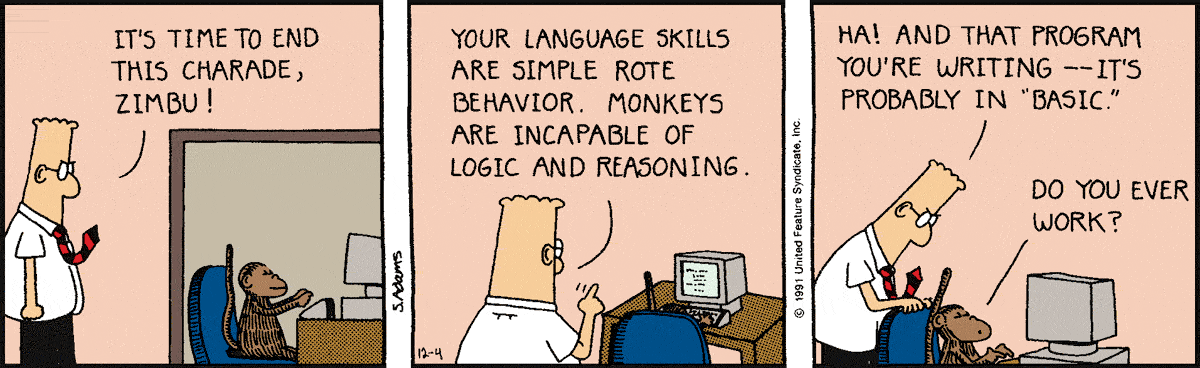
\includegraphics[width=\textwidth]{figs/dilbert-1991-12-04.png}

The invention of the PC, which democratized computing, owes its success
to two important inventions.  
The first occurred in 1971, when engineer Ted Hoff and others
at Intel invented the 4004 microprocessor.
The microprocessor industry's ability to exploit Moore's Law resulted in
the 4004 evolving to the 8080 in 1974---the microprocessor that powered
the first hobbyist PC, the Altair---and subsequently the 8086 in 1976,
the direct  ancestor of today's ubiquitous x86
architecture.
The second invention is the creation and rapid dissemination of the
high-level introductory programming language BASIC.

Before universities had computers that were widely accessible to students, BASIC
provided a kinder, gentler introduction to computing suitable for
everyone, especially nontechnical majors.
Before there was such a thing as a PC software industry, 
BASIC allowed early hobbyists to quickly get started writing their own
programs.
Before computer games became a multibillion-dollar industry, beginning
programmers and hobbyists were writing their own games in BASIC, to
exploit the rapidly-developing capabilities of graphics and sound on
early PCs. 
Much of the other software that fueled the PC revolution---online
bulletin boards, simple utilities, small-business software---was written
in BASIC. 
As science fiction author David Brin has written~\cite{why_johnny_cant_code},
despite its flaws, BASIC
was sufficiently nonthreatening to introduce an entire generation of
newbies to the joy of programming.

Today's world-class universities boast that over 90\% of all
undergraduates are exposed to introductory programming, and movements
like ``CS for all'' and sites like \T{code.org} aim to expose everyone
to coding.
Dartmouth College, where BASIC was invented, had largely
achieved this by 1971 on its campus~\cite{man_and_computer} by implementing the
farsighted vision of BASIC's creators.
A wide supporting cast of characters---idealistic professors,
ambitious entrepreneurs, garage hobbyists, community-minded
professionals, and the companies and institutions where they
worked---introduced  an entire generation
of hobbyist programmers to the joy of programming using BASIC.

Yet quotes like Dijkstra's suggest that despite its pivotal role in the PC
revolution, BASIC is probably one of the most maligned programming
languages to achieve widespread use.  It's time the true story of
BASIC's influence was told.
